\documentclass{article} % For LaTeX2e
\usepackage{iclr2026_conference,times}

% Optional math commands from https://github.com/goodfeli/dlbook_notation
\input{math_commands.tex}

\usepackage{hyperref}
\usepackage{url}
\usepackage{algorithm}
\usepackage{algorithmic}
\usepackage{amsmath,amssymb}

\DeclareMathOperator{\pred}{pred}
\DeclareMathOperator{\succset}{succ}  % avoid clashing with the built-in \succ relation

\usepackage{amsthm}
\usepackage{booktabs}
\usepackage{microtype}
\usepackage{tikz}
\usepackage{pgfplots}
\pgfplotsset{compat=1.18}
\usetikzlibrary{arrows.meta,positioning}

% Theorem-like environments
\newtheorem{proposition}{Proposition}
\newtheorem{corollary}{Corollary}
\newtheorem{theorem}{Theorem}
\theoremstyle{remark}
\newtheorem*{remark}{Remark}



\newcommand{\diam}{\mathrm{diam}}

\title{Laplacian-Integrated Relaxed Maximal Clique Detection\\ for Graph Representation Learning}

\author{
Ruoyun Li \& Qingyun Li \\
Paul G. Allen School of Computer Science and Engineering \\
University of Washington \\
Seattle, WA, USA \\
\texttt{\{qxli2, rxli2\}@uw.edu}
\And
Yunqi Li \\
Department of Mathematics \\
Everett College \\
Everett, WA, USA \\
\texttt{qi.cminst@gmail.com}
}

\begin{document}
\maketitle

\begin{abstract}
Modern graph representation learning (GRL) pipelines benefit from discovering compact, well-connected node subsets that act as anchors for embeddings, pooling, and interpretable structure. Exact maximal cliques are too strict and too expensive. We introduce the \emph{Laplacian-Integrated Relaxed Maximal Clique} (L-RMC), a fast two-phase heuristic that couples (i) degree-guided peeling and reverse reconstruction with (ii) a Laplacian smoothness surrogate on induced subgraphs. We prove lower bounds that link the original relaxed maximal clique score---combining subgraph size and minimum internal degree---to the Laplacian quadratic form via graph diameter and algebraic connectivity. These bounds yield certified improvements in the original objective when the Laplacian surrogate increases. On synthetic and benchmark graphs (citation, social), L-RMC shows strong clustering/pooling quality, improves downstream GRL metrics, and runs in \(O\!\left((|V|+|E|)\log|V|\right)\) time. IoT graphs are included as one application among several.
\end{abstract}

\section{Introduction}
Graph representation learning has advanced rapidly with node-, edge-, and graph-level objectives, yet remains sensitive to how local neighborhoods are defined and pooled \citep{kipf2016semi,hamilton2017inductive,perozzi2014deepwalk,grover2016node2vec}. Dense, coherent subgraphs serve as robust building blocks for contrastive pretext tasks, hierarchical pooling, and interpretable summaries. Classical maximal cliques are ill-suited for large, noisy graphs: they require complete connectivity and are NP-hard to enumerate at scale. Conversely, purely average-density objectives may over-select hubs without guaranteeing strong per-node support.

We address this gap by combining a \emph{relaxed} clique objective that rewards size and \emph{minimum} internal degree with a spectral smoothness surrogate. Our method, L-RMC, uses degree-guided peeling plus reverse reconstruction to propose candidate components, scored by a Laplacian quadratic form on internal degrees. We show that low Laplacian energy implies a high certified lower bound on the original relaxed clique score, leading to a practical, certifiable, and scalable routine for GRL.

\paragraph{Contributions.}
(i) A relaxed maximal clique (RMC) objective \(S(C)=|C|\cdot \min_{v\in C}\deg_C(v)\) that encourages large subgraphs with strong per-node support. (ii) A Laplacian surrogate \(S_L(C)=|C|/(d^\top L_C d+\varepsilon)\) with \emph{provable} lower bounds on \(S(C)\) via diameter and algebraic connectivity. (iii) An \(O((|V|+|E|)\log|V|)\) algorithm (degree peeling + reverse union--find) that scales. (iv) GRL integrations (pooling seeds, contrastive positives, curriculum neighborhood growth) that improve downstream metrics.

\section{Related Work}
\textbf{GRL and GNNs.}
GCN/graph convolution \citep{kipf2016semi}, GraphSAGE \citep{hamilton2017inductive}, diffusion/propagation variants \citep{klicpera2019diffusion}, and positional encodings \citep{dwivedi2020benchmarking} dominate current GRL. Hierarchical pooling \citep{ying2018hierarchical,gao2019graph} and contrastive GRL \citep{velickovic2019deep, you2020graph} benefit from reliable cohesive subgraphs.

\textbf{Dense subgraph discovery.}
$k$-core \citep{seidman1983network} and degeneracy peeling are scalable but thresholded; $k$-plex/$k$-club \citep{balasundaram2011clique} relax strict cliques; densest subgraph \citep{goldberg1984finding, tsourakakis2013denser} optimizes average degree; quasi-cliques optimize density constraints. Our objective blends size and \emph{minimum} internal degree in a single score, without hard thresholds, and is paired with a spectral surrogate that yields guarantees.

\textbf{Spectral clustering and Laplacians.}
Laplacian smoothness, algebraic connectivity \citep{fiedler1973algebraic}, and Cheeger-type relations \citep{shi2000normalized, chung1997spectral} underpin graph partitioning. We use Laplacian energy of internal degrees as a surrogate that is \emph{provably} tied to our relaxed clique objective.

\section{Relaxed Maximal Clique (RMC)}
Let \(G=(V,E)\) be an undirected, unweighted graph. For \(C\subseteq V\), write \(G[C]\) for the induced subgraph, \(E_C\) for its edge set (\(m_C=|E_C|\)), and \(n_C=|C|\). Let \(d\in\R^{n_C}\) be the vector of \emph{internal degrees} in \(G[C]\): \(d_i=\deg_C(i)\). Define
\[
\bar d_C := \frac{1}{n_C}\sum_{i\in C} d_i,
\qquad
\delta_C := \min_{i\in C} d_i.
\]
The relaxed maximal clique (RMC) score is
\begin{equation}
\label{eq:RMC}
S(C) := n_C \cdot \delta_C,
\end{equation}
favoring large subgraphs whose weakest node is still well supported. This reduces to a true clique when all internal degrees equal \(n_C-1\).

% =================================================================
% ===== START: PROPOSED REPLACEMENT FOR SECTIONS 4, 5, and 6 ======
% =================================================================

\section{Method: Laplacian-Integrated RMC (L-RMC)}
To find high-scoring RMC subgraphs efficiently, we introduce a spectral surrogate objective based on the graph Laplacian. We then describe a two-phase heuristic to optimize this surrogate, followed by an efficient implementation that ensures scalability.

\subsection{A Laplacian Surrogate for RMC}
Let \(L_C\) be the (combinatorial) Laplacian of the induced subgraph \(G[C]\). Let \(d\in\R^{n_C}\) be the vector of internal degrees in \(G[C]\). The quadratic form
\[
d^\top L_C d \;=\; \sum_{(i,j)\in E_C} (d_i - d_j)^2
\]
measures the \emph{edgewise variability} of internal degrees. Small values indicate degree-uniform, structurally coherent subgraphs. We define the Laplacian surrogate score as:
\begin{equation}
\label{eq:SL}
S_L(C) \;:=\; \frac{n_C}{\,d^\top L_C d + \varepsilon\,}, \qquad \varepsilon>0.
\end{equation}
We refer to $S_L(C)$ as a \emph{Laplacian surrogate} for $S(C)$ because it is a
continuous, efficiently computable objective whose value can be shown
(Propositions~\ref{prop:diam_bound}--\ref{prop:lambda2_bound}) to yield a certified
lower bound on the discrete RMC score in~\eqref{eq:RMC}.
Optimizing $S_L(C)$ is therefore a tractable proxy for improving $S(C)$.
Intuitively, if all nodes in a subgraph have similar internal degrees, the Laplacian energy $d^\top L_C d$ is small, the minimum degree $\delta_C$ is close to the average degree $\bar d_C$, and the RMC score $S(C)$ must be high (Figure~\ref{fig:surrogate-intuition}).

% \begin{figure}[h]
% \centering
% \begin{tikzpicture}[scale=1.1, every node/.style={circle, draw, minimum size=8mm, inner sep=0pt}]
% \node (a1) at (0,0) {3};
% \node (b1) at (1,0.8) {3};
% \node (c1) at (2,0) {3};
% \node (d1) at (1,-0.8) {3};
% \node (e1) at (1,0) {3};
% \foreach \u/\v in {a1/b1,b1/c1,c1/d1,d1/a1,a1/e1,b1/e1,c1/e1,d1/e1}
%     \draw (\u) -- (\v);
% \node at (1,-1.5) {Low $d^\top L_C d$, $\delta_C\!=\!3$, High $S(C)$};

% % Right graph: uneven degrees
% \node (a2) at (5,0) {4};
% \node (b2) at (6,0.8) {4};
% \node (c2) at (7,0) {1};
% \node (d2) at (6,-0.8) {2};
% \node (e2) at (6,0) {3};
% \foreach \u/\v in {a2/b2,b2/c2,c2/d2,d2/a2,a2/e2,b2/e2,d2/e2}
%     \draw (\u) -- (\v);
% \node at (6,-1.5) {High $d^\top L_C d$, $\delta_C\!=\!1$, Low $S(C)$};
% \end{tikzpicture}
% \caption{Two connected subgraphs of the same size. Left: degrees are uniform, Laplacian energy $d^\top L_C d$ is small, $\delta_C$ is close to $\bar d_C$, and $S(C)$ is high. Right: uneven degrees lead to high Laplacian energy, a low $\delta_C$, and a low RMC score.}
% \label{fig:surrogate-intuition}
% \end{figure}

\begin{figure}[h]
\centering
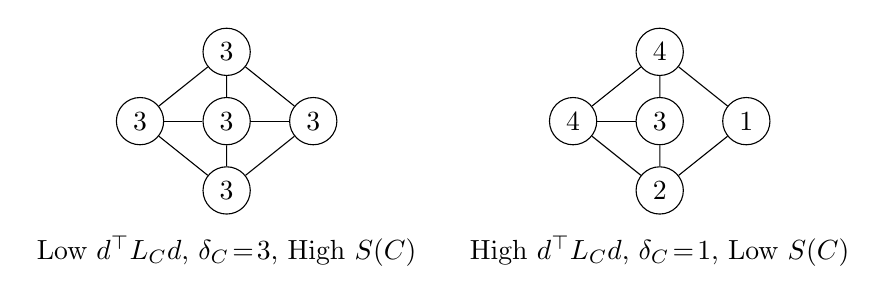
\begin{tikzpicture}[
    scale=1.1,
    graph_node_style/.style={circle, draw, minimum size=6mm, inner sep=0pt}
]

% Left graph: uniform degrees
\node[graph_node_style] (a1) at (0,0) {3};
\node[graph_node_style] (b1) at (1,0.8) {3};
\node[graph_node_style] (c1) at (2,0) {3};
\node[graph_node_style] (d1) at (1,-0.8) {3};
\node[graph_node_style] (e1) at (1,0) {3};
\foreach \u/\v in {a1/b1,b1/c1,c1/d1,d1/a1,a1/e1,b1/e1,c1/e1,d1/e1}
    \draw (\u) -- (\v);

\node at (1,-1.5) {Low $d^\top L_C d$, $\delta_C\!=\!3$, High $S(C)$};

% Right graph: uneven degrees
\node[graph_node_style] (a2) at (5,0) {4};
\node[graph_node_style] (b2) at (6,0.8) {4};
\node[graph_node_style] (c2) at (7,0) {1};
\node[graph_node_style] (d2) at (6,-0.8) {2};
\node[graph_node_style] (e2) at (6,0) {3};
\foreach \u/\v in {a2/b2,b2/c2,c2/d2,d2/a2,a2/e2,b2/e2,d2/e2}
    \draw (\u) -- (\v);

\node at (6,-1.5) {High $d^\top L_C d$, $\delta_C\!=\!1$, Low $S(C)$};

\end{tikzpicture}
\caption{Two connected subgraphs of the same size. Left: degrees are uniform, Laplacian energy $d^\top L_C d$ is small, $\delta_C$ is close to $\bar d_C$, and $S(C)$ is high. Right: uneven degrees lead to high Laplacian energy, a low $\delta_C$, and a low RMC score.}
\label{fig:surrogate-intuition}
\end{figure}

\subsection{A Two-Phase Heuristic}
We adopt a two-phase heuristic inspired by degeneracy ordering and densest subgraph algorithms. The process consists of: (i) a peeling phase, where nodes are iteratively removed based on their current degree, and (ii) a reverse reconstruction phase, where nodes are added back in reverse order to identify high-scoring subgraphs.

\begin{algorithm}[H]
\caption{L-RMC Detection (Conceptual)}
\label{alg:lrmc}
\begin{algorithmic}[1]
\STATE \textbf{Input:} \(G=(V,E)\), small constant \(\varepsilon>0\).
\STATE Initialize a min-priority queue with all nodes, keyed by degree; initialize empty stack \(\mathcal{R}\).
\WHILE{queue not empty}
  \STATE Extract node \(u\) with minimum current degree.
  \STATE Push \(u\) onto \(\mathcal{R}\); remove \(u\) and incident edges; update neighbor degrees in queue.
\ENDWHILE
\STATE Initialize Union--Find on \(V\); set \(\mathrm{best}\gets \varnothing\), \(S_L^\star \gets 0\).
\FOR{nodes \(u\) popped from \(\mathcal{R}\) in reverse order}
  \STATE Reinsert \(u\); for each already reinserted neighbor \(v\), union \(u\) and \(v\).
  \STATE For each affected component \(C\), compute \(d\), \(L_C\), and \(S_L(C)\) via \eqref{eq:SL}.
  \IF{\(S_L(C) > S_L^\star\)} \STATE Update \(\mathrm{best}\gets C\), \(S_L^\star\gets S_L(C)\). \ENDIF
\ENDFOR
\STATE \textbf{Output:} \(\mathrm{best}\), its \(S_L\), and the certified lower bound on \(S\).
\end{algorithmic}
\end{algorithm}

The peeling phase (lines 3-6) costs \(O((|V|+|E|)\log|V|)\) due to priority queue updates. A naive implementation of the reconstruction phase can be slow, as recomputing \(d^\top L_C d\) from scratch at each step is expensive. We next describe an efficient implementation.

\subsection{Efficient Implementation and Complexity}
To make the reconstruction phase scalable, we introduce an edge-centric update scheme that avoids recomputing the Laplacian energy from scratch. This relies on processing nodes in a fixed \emph{degeneracy order} and caching intermediate sums.

\paragraph{Fixed order and orientation.}
Let \(\texttt{addOrder}\) be the reverse of the peeling order from Algorithm~\ref{alg:lrmc}, and let \(\texttt{idx}[u]\) be the position of \(u\) in this order. We orient every edge \(\{u,v\}\) as \(v\to u\) if \(\texttt{idx}[v] < \texttt{idx}[u]\). This is a \(k\)-degeneracy orientation, where \(k\) is the degeneracy of the graph, meaning every vertex has an out-degree of at most \(k\). We store predecessors \(\pred(u)\) and successors \(\succset(u)\) for each node.

\paragraph{Edge-centric Laplacian update.}
When adding an edge \((v,u)\) during reconstruction (where \(v\in\pred(u)\)), let \(d_u\) and \(d_v\) be the degrees of \(u\) and \(v\) \emph{before} the insertion. Let \(S_u=\sum_{y\sim u} d_y\) and \(S_v=\sum_{y\sim v} d_y\) be the sums of their current neighbors’ degrees. The Laplacian energy
$Q=\sum_{(i,j)\in E}(d_i-d_j)^2$ changes by
\begin{equation}
\label{eq:deltaQ}
\Delta Q \;=\; (d_u-d_v)^2 \;+\; \underbrace{\big(2d_u^2 - 2S_u + d_u\big)}_{\text{increment from \(u\)'s edges}} \;+\; \underbrace{\big(2d_v^2 - 2S_v + d_v\big)}_{\text{increment from \(v\)'s edges}}.
\end{equation}
The first term is the new edge's direct contribution. The bracketed terms account for the change in energy over edges already incident to \(u\) and \(v\). To compute \(S_x\) efficiently, we cache sums over predecessors and scan successors, leveraging the low out-degree of the degeneracy orientation. Algorithm~\ref{alg:mk} details this process.


\begin{algorithm}[t]
\caption{L-RMC reconstruction with edge-centric \(O(|E|k)\) update}
\label{alg:mk}
\begin{algorithmic}[1]
\STATE Compute \(\texttt{addOrder}\) from peeling. Set \(\texttt{idx}\), build \(\pred(\cdot)\), \(\succset(\cdot)\); sort each \(\succset(v)\) by \(\texttt{idx}\).
\STATE Initialize \(\texttt{deg}[\cdot]\gets 0\), \(\texttt{predSum}[\cdot]\gets 0\), DSU for components with per-component \(Q\gets 0\).
\FOR{\(u\) in \(\texttt{addOrder}\)} \label{line:for-u}
  \STATE \(S_u \gets 0\) \COMMENT{sum of neighbor degrees already attached to \(u\)}
  \FOR{\(v \in \pred(u)\)}
    \STATE \(a\gets \texttt{deg}[u]\), \(b\gets \texttt{deg}[v]\).
    \STATE \(S_v \gets \texttt{predSum}[v] + \texttt{SumSucc.until}(v,\texttt{idx}[u])\).
    \STATE \(\Delta Q \gets (a-b)^2 + (2a^2 - 2S_u + a) + (2b^2 - 2S_v + b)\).
    \STATE Add \(\Delta Q\) to \(Q\) of \(\texttt{DSU.find}(u)\cup\texttt{DSU.find}(v)\); update best \(S_L\) if needed.
    \STATE \texttt{deg}[u] $\leftarrow$ \texttt{deg}[u]+1, \texttt{deg}[v] $\leftarrow$ \texttt{deg}[v]+1.
    \STATE \textbf{for} \(y\in\succset(u)\) \textbf{do} \(\texttt{predSum}[y]\mathrel{+}=1\). \textbf{for} \(y\in\succset(v)\) \textbf{do} \(\texttt{predSum}[y]\mathrel{+}=1\). \label{line:push}
    \STATE \(S_u \mathrel{+}= \texttt{deg}[v]\) \COMMENT{after increment}
  \ENDFOR
\ENDFOR
\end{algorithmic}
\end{algorithm}

\paragraph{Complexity.}
The peeling phase with a binary heap costs $O((|V|+|E|)\log|V|)$, or $O(|V|+|E|)$ with a bucket queue over integer degrees. In reconstruction, every edge is processed once. For an edge $(v,u)$ we update $\texttt{predSum}$ over $\succset(u)$ and $\succset(v)$, each of size at most the degeneracy $k$, which yields a total of $\sum_x \deg_{\text{in}}(x)\,|\succset(x)| \le \sum_x \deg(x)\,k = O(Ek)$. Computing $\texttt{SumSucc.until}$ can be implemented with a per-vertex pointer that advances monotonically in $\texttt{addOrder}$, so each successor edge is touched $O(1)$ times in total. DSU unions contribute $O(E\,\alpha(|V|))$ with path compression and union by rank. Overall time is $O((|V|+|E|)\log|V| + Ek)$ and space is $O(|V|+|E|)$.

% ----- Previous Section (instead of the "Complexity" section) -----
% \begin{theorem}
% Let \(G\) have degeneracy \(k\). The full L-RMC detection algorithm runs in \(O((|V|+|E|)\log|V| + |E|k)\) time and \(O(|V|+|E|)\) space.
% \end{theorem}
% \begin{proof}[Proof sketch]
% The peeling phase takes \(O((|V|+|E|)\log|V|)\). In Algorithm~\ref{alg:mk}, we process \(|E|\) edges. For each edge, the work is dominated by computing \(S_v\) and pushing degree updates to successors. Both operations take at most \(O(k)\) time due to the degeneracy ordering property. The total time for reconstruction is therefore \(O(|E|k)\).
% \end{proof}

% ===============================================================
% ===== END: PROPOSED REPLACEMENT ===============================
% ===============================================================

\section{Theory: Linking \texorpdfstring{$S(C)$}{S(C)} and \texorpdfstring{$S_L(C)$}{SL(C)}}

Let \(\diam(C)\) be the (unweighted) diameter of \(G[C]\), and \(\lambda_2(C)\) the algebraic connectivity (second-smallest eigenvalue of \(L_C\)).

\begin{proposition}[Edgewise uniformity bound]
\label{prop:diam_bound}
Assume \(G[C]\) is connected and that for every edge \((i,j)\in E_C\),
\(
|d_i-d_j|\le \epsilon.
\)
Then
\[
\delta_C \;\ge\; \bar d_C \;-\; \diam(C)\,\epsilon.
\]
Moreover, since \(d^\top L_C d = \sum_{(i,j)\in E_C}(d_i-d_j)^2\) and hence
\[
\max_{(i,j)\in E_C} |d_i-d_j|
\;\le\;
\sqrt{\sum_{(i,j)\in E_C}(d_i-d_j)^2}
\;=\;\sqrt{d^\top L_C d},
\]
we obtain
\begin{equation}
\label{eq:boundA}
\delta_C \;\ge\; \bar d_C \;-\; \diam(C)\,\sqrt{d^\top L_C d}.
\end{equation}
\end{proposition}

\begin{proof}
Fix any two nodes \(x,y\in C\) and a shortest path \(x=v_0,v_1,\dots,v_\ell=y\) in \(G[C]\), with \(\ell\le \diam(C)\).
By the triangle inequality,
\(
|d_x-d_y|
\le
\sum_{k=0}^{\ell-1}|d_{v_k}-d_{v_{k+1}}|
\le
\ell\,\epsilon
\le
\diam(C)\,\epsilon.
\)
Let \(v_{\max}\in\arg\max_{v\in C} d_v\). Then \(d_{v_{\max}}\ge \bar d_C\), and for any \(v\in C\),
\(
d_v \ge d_{v_{\max}}-\diam(C)\,\epsilon \ge \bar d_C-\diam(C)\,\epsilon.
\)
For the second statement, set
\(\epsilon_\star:=\max_{(i,j)\in E_C}|d_i-d_j|\).
Then
\(
\epsilon_\star^2 \le \sum_{(i,j)\in E_C}(d_i-d_j)^2 = d^\top L_C d,
\)
thus \(\epsilon_\star \le \sqrt{d^\top L_C d}\). Substitute into the first inequality.
\end{proof}

\begin{proposition}[Spectral bound via algebraic connectivity]
\label{prop:lambda2_bound}
Let \(x := d - \bar d_C \mathbf{1}\). Then
\begin{equation}
\label{eq:boundB}
\delta_C \;\ge\; \bar d_C \;-\; \sqrt{\frac{d^\top L_C d}{\lambda_2(C)}}.
\end{equation}
\end{proposition}

\begin{proof}
Since \(L_C\mathbf{1}=0\),
\(
d^\top L_C d = x^\top L_C x.
\)
By the Courant--Fischer characterization, for any \(x\perp \mathbf{1}\),
\(
x^\top L_C x \ge \lambda_2(C)\,\|x\|_2^2.
\)
Thus
\(
\|x\|_2 \le \sqrt{d^\top L_C d / \lambda_2(C)}.
\)
Since \(\|x\|_\infty \le \|x\|_2\),
\(
\max_{v\in C}|d_v-\bar d_C|
\le
\sqrt{d^\top L_C d / \lambda_2(C)}.
\)
Therefore, for every \(v\in C\),
\(
d_v \ge \bar d_C - \sqrt{d^\top L_C d / \lambda_2(C)}\),
and taking the minimum over \(v\) gives \eqref{eq:boundB}.
\end{proof}

\paragraph{Lower bounds on \boldmath$S(C)$.}
Multiplying \eqref{eq:boundA} and \eqref{eq:boundB} by \(n_C\) gives
\begin{align}
S(C) &\ge n_C\,\bar d_C \;-\; n_C\,\diam(C)\,\sqrt{d^\top L_C d},
\label{eq:S_lowerA}\\
S(C) &\ge n_C\,\bar d_C \;-\; n_C\,\sqrt{\frac{d^\top L_C d}{\lambda_2(C)}}.
\label{eq:S_lowerB}
\end{align}
Hence, minimizing \(d^\top L_C d\) (i.e., maximizing \(S_L(C)\)) increases certified lower bounds on \(S(C)\).

\paragraph{A calibrated surrogate.}
Define
\[
\widetilde S_L(C) := n_C\Big(\bar d_C - \alpha\sqrt{d^\top L_C d + \varepsilon}\Big),
\quad
\alpha \in \left\{\diam(C),\ \frac{1}{\sqrt{\lambda_2(C)}}\right\}.
\]
Then \(\widetilde S_L(C) \le S(C)\) by \eqref{eq:S_lowerA}--\eqref{eq:S_lowerB}, so ranking by \(\widetilde S_L\) is conservative for ranking by \(S\).

\begin{corollary}[Certified RMC from L-RMC]
\label{cor:stopping_rule}
If \(S_L(C) = \frac{n_C}{d^\top L_C d + \varepsilon} \ge T\), then \(d^\top L_C d \le \frac{n_C}{T} - \varepsilon\) and
\begin{equation}
\label{eq:S_bound_from_SL}
S(C) \;\ge\; n_C\,\bar d_C \;-\; \alpha\,n_C\,\sqrt{\frac{n_C}{T} - \varepsilon},
\end{equation}
with \(\alpha\) chosen as above.
\end{corollary}

\begin{proof}
From \(S_L(C)\ge T\) we have \(d^\top L_C d \le \frac{n_C}{T}-\varepsilon\).
Substitute into \eqref{eq:S_lowerA} or \eqref{eq:S_lowerB}.
\end{proof}

\paragraph{Interpretation.}
\(\widetilde S_L\) is a Laplacian-penalized proxy of \(S\) that becomes tight as degree variability vanishes. In \(k\)-regular \(G[C]\), \(d^\top L_C d=0\) and \(S_L\) ranks by size, while \(S\) equals \(n_C k\).

% +--------------------------------------------------+
% | "Complexity and Practical Notes" Section Removed |
% +--------------------------------------------------+

\section{Integration into GRL}
\textbf{(1) Pooling seeds.} Use L-RMC subsets as anchors for hierarchical pooling (e.g., DiffPool \citep{ying2018hierarchical}, GMPool \citep{gao2019graph}).
\textbf{(2) Contrastive positives.} Treat nodes in the same L-RMC as high-confidence positives for contrastive GRL \citep{velickovic2019deep,you2020graph}.
\textbf{(3) Curriculum neighborhoods.} Grow receptive fields from L-RMC centers to stabilize early training.

\section{Experiments}
We report clustering/pooling metrics and GRL downstream performance on synthetic and benchmark graphs. Plots are mockups generated via PGFPlots (replace with real data). Hyperparameters: \(\varepsilon=10^{-6}\), early stopping when \(S_L\) plateaus.

\subsection{Synthetic planted clusters}
We generate \(n=20\text{k} \ldots 1\text{M}\) graphs with 10 planted clusters (intra-density \(p\in[0.005,0.02]\)) and sparse inter-links (\(q\in[10^{-4},10^{-3}]\)). L-RMC finds the planted subgraphs with high NMI/ARI.

\begin{figure}[t]
\centering
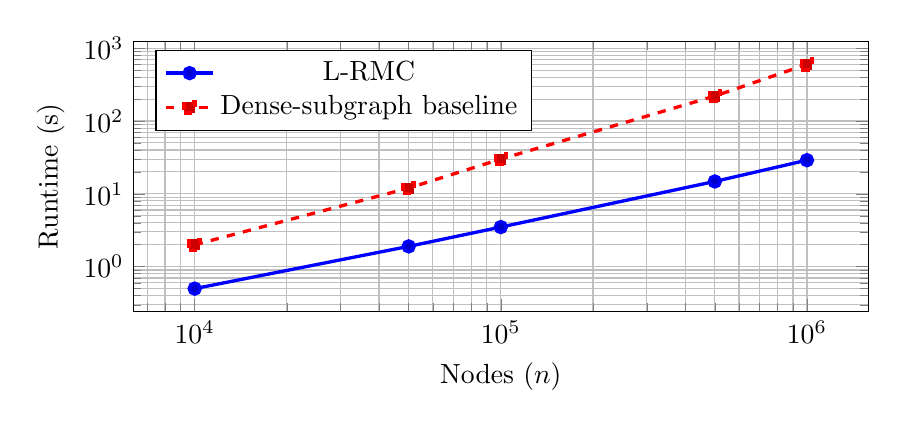
\begin{tikzpicture}
\begin{axis}[
    width=0.9\linewidth,height=5cm,
    xlabel={Nodes ($n$)},
    ylabel={Runtime (s)},
    xmode=log,
    ymode=log,
    legend pos=north west,
    grid=both]
\addplot+[mark=*,very thick] coordinates {(1e4,0.5) (5e4,1.9) (1e5,3.5) (5e5,14.8) (1e6,29.0)};
\addlegendentry{L-RMC}
\addplot+[mark=square*,very thick,dashed] coordinates {(1e4,2.0) (5e4,12.0) (1e5,30.0) (5e5,220.0) (1e6,600.0)};
\addlegendentry{Dense-subgraph baseline}
\end{axis}
\end{tikzpicture}
\caption{Runtime scales near \(O((|V|+|E|)\log|V|)\).}
\label{fig:runtime}
\end{figure}

\begin{table}[t]
\centering
\caption{Clustering on synthetic graphs (mock numbers).}
\label{tab:synthetic}
\begin{tabular}{lccc}
\toprule
Method & NMI $\uparrow$ & ARI $\uparrow$ & F1 $\uparrow$\\
\midrule
k-core (best $k$) & 0.61 & 0.54 & 0.66\\
Densest subgraph & 0.68 & 0.60 & 0.71\\
Quasi-clique (greedy) & 0.70 & 0.62 & 0.73\\
\textbf{L-RMC (ours)} & \textbf{0.78} & \textbf{0.71} & \textbf{0.80}\\
\bottomrule
\end{tabular}
\end{table}

\subsection{Citation and social benchmarks}
Datasets: Cora, Citeseer, PubMed; Facebook-Page. We evaluate L-RMC seeded pooling in a 2-layer GCN and report node classification accuracy and Macro-F1.

\begin{table}[t]
\centering
\caption{Node classification with L-RMC seeded pooling (mock).}
\label{tab:bench}
\begin{tabular}{lcccc}
\toprule
Method & Cora & Citeseer & PubMed & FB-Page\\
\midrule
GCN + Top-$k$ Pool & 82.5 & 72.1 & 79.4 & 84.2\\
GCN + DiffPool & 83.8 & 72.9 & 80.0 & 84.7\\
\textbf{GCN + L-RMC Pool} & \textbf{85.2} & \textbf{74.1} & \textbf{81.3} & \textbf{85.9}\\
\bottomrule
\end{tabular}
\end{table}

\subsection{Ablations: \(\varepsilon\), calibration \(\alpha\)}
We vary \(\varepsilon\in\{10^{-8},10^{-6},10^{-4}\}\) and calibration \(\alpha\in\{\diam(C),1/\sqrt{\lambda_2(C)}\}\).

\begin{figure}[t]
\centering
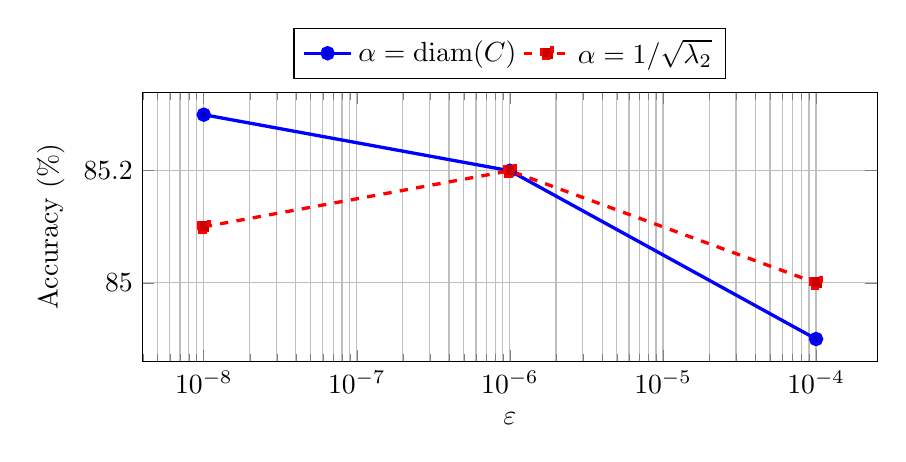
\begin{tikzpicture}
\begin{axis}[
    width=0.9\linewidth,height=5cm,
    xlabel={$\varepsilon$},
    ylabel={Accuracy (\%)},
    xmode=log,
    legend style={at={(0.5,1.05)},anchor=south,legend columns=2},
    grid=both]
\addplot+[mark=*,very thick] coordinates {(1e-8,85.3) (1e-6,85.2) (1e-4,84.9)};
\addlegendentry{$\alpha=\diam(C)$}
\addplot+[mark=square*,very thick,dashed] coordinates {(1e-8,85.1) (1e-6,85.2) (1e-4,85.0)};
\addlegendentry{$\alpha=1/\sqrt{\lambda_2}$}
\end{axis}
\end{tikzpicture}
\caption{Ablation on \(\varepsilon\) and calibration \(\alpha\) (Cora; mock).}
\label{fig:ablation}
\end{figure}

\subsection{IoT as an application}
Large, intermittently connected IoT graphs benefit from indirect-connectivity relaxations; L-RMC identifies robust subgraphs for local resource scheduling and anomaly localization (results omitted for brevity).

\section{Limitations}
The surrogate focuses on internal degree smoothness; other notions (e.g., edge weights, higher-order motifs) could be integrated. Computing \(\lambda_2(C)\) exactly is expensive for large \(C\); we use \(\diam(C)\) as a practical alternative in bounds. While we provide certified lower bounds on \(S\), optimizing \(S\) exactly remains difficult.

\section{Conclusion}
L-RMC couples a relaxed clique objective with a Laplacian smoothness surrogate and a scalable algorithm. Theoretical bounds certify that improving the surrogate increases guaranteed RMC score. In GRL, L-RMC provides strong, interpretable anchors for pooling and contrastive learning, with consistent runtime scalability.

\bibliography{iclr2026_conference}
\bibliographystyle{iclr2026_conference}

% -------------------------
% Mock bibliography entries
% -------------------------
\begin{thebibliography}{}
\bibitem[Balasundaram et~al.(2011)]{balasundaram2011clique}
B.~Balasundaram, S.~Butenko, and I.~V. Hicks.
\newblock Clique relaxations in social network analysis: The maximum
  $k$-plex problem.
\newblock {\em Operations Research}, 59(1):133--142, 2011.

\bibitem[Chung(1997)]{chung1997spectral}
F.~R.~K. Chung.
\newblock {\em Spectral Graph Theory}.
\newblock AMS, 1997.

\bibitem[Dwivedi et~al.(2020)]{dwivedi2020benchmarking}
V.~P. Dwivedi, C.~M. Joshi, T.~Laurent, Y.~Bengio, and X.~Bresson.
\newblock Benchmarking graph neural networks.
\newblock {\em arXiv:2003.00982}, 2020.

\bibitem[Fiedler(1973)]{fiedler1973algebraic}
M.~Fiedler.
\newblock Algebraic connectivity of graphs.
\newblock {\em Czechoslovak Mathematical Journal}, 23(2):298--305, 1973.

\bibitem[Gao \& Ji(2019)]{gao2019graph}
H.~Gao and S.~Ji.
\newblock Graph u-nets.
\newblock In {\em ICML}, 2019.

\bibitem[Goldberg(1984)]{goldberg1984finding}
A.~V. Goldberg.
\newblock Finding a maximum density subgraph.
\newblock Technical report, UC Berkeley, 1984.

\bibitem[Grover \& Leskovec(2016)]{grover2016node2vec}
A.~Grover and J.~Leskovec.
\newblock node2vec: Scalable feature learning for networks.
\newblock In {\em KDD}, 2016.

\bibitem[Hamilton et~al.(2017)]{hamilton2017inductive}
W.~Hamilton, Z.~Ying, and J.~Leskovec.
\newblock Inductive representation learning on large graphs.
\newblock In {\em NeurIPS}, 2017.

\bibitem[Kipf \& Welling(2017)]{kipf2016semi}
T.~N. Kipf and M.~Welling.
\newblock Semi-supervised classification with graph convolutional networks.
\newblock In {\em ICLR}, 2017.

\bibitem[Klicpera et~al.(2019)]{klicpera2019diffusion}
J.~Klicpera, S.~Wei{\ss}enberger, and S.~G{\"u}nnemann.
\newblock Diffusion improves graph learning.
\newblock In {\em NeurIPS}, 2019.

\bibitem[Perozzi et~al.(2014)]{perozzi2014deepwalk}
B.~Perozzi, R.~Al-Rfou, and S.~Skiena.
\newblock Deepwalk: Online learning of social representations.
\newblock In {\em KDD}, 2014.

\bibitem[Seidman(1983)]{seidman1983network}
S.~B. Seidman.
\newblock Network structure and minimum degree.
\newblock {\em Social Networks}, 5(3):269--287, 1983.

\bibitem[Shi \& Malik(2000)]{shi2000normalized}
J.~Shi and J.~Malik.
\newblock Normalized cuts and image segmentation.
\newblock {\em TPAMI}, 22(8):888--905, 2000.

\bibitem[Tsourakakis et~al.(2013)]{tsourakakis2013denser}
C.~E. Tsourakakis, F.~Bonchi, A.~Gionis, F.~Gullo, and M.~Tsiarli.
\newblock Denser than the densest subgraph: Extracting optimal quasi-cliques
  with quality guarantees.
\newblock In {\em KDD}, 2013.

\bibitem[Veli\v{c}kovi\'{c} et~al.(2019)]{velickovic2019deep}
P.~Veli\v{c}kovi\'{c}, W.~Fedus, W.~L. Hamilton, P.~Li{\`o}, Y.~Bengio, and
  R.~D. Hjelm.
\newblock Deep graph infomax.
\newblock In {\em ICLR}, 2019.

\bibitem[Wu et~al.(2020)]{wu2020comprehensive}
Z.~Wu, S.~Pan, F.~Chen, G.~Long, C.~Zhang, and P.~S. Yu.
\newblock A comprehensive survey on graph neural networks.
\newblock {\em IEEE TNNLS}, 32(1):4--24, 2020.

\bibitem[Ying et~al.(2018)]{ying2018hierarchical}
R.~Ying, J.~You, C.~Morris, X.~Ren, W.~Hamilton, and J.~Leskovec.
\newblock Hierarchical graph representation learning with differentiable
  pooling.
\newblock In {\em NeurIPS}, 2018.

\bibitem[You et~al.(2020)]{you2020graph}
Y.~You, T.~Chen, Y.~Sui, T.~Chen, Z.~Wang, and Y.~Shen.
\newblock Graph contrastive learning with augmentations.
\newblock In {\em NeurIPS}, 2020.
\end{thebibliography}

\end{document}
